\documentclass[a4paper, 12pt]{article}

	\usepackage[utf8]{inputenc}
	\usepackage[T1]{fontenc}
	\usepackage{amsmath}
	\usepackage{graphicx}
	\usepackage{url}

    \title{Electroacoustic Project\\IMDEA Master 2}
    \author{B. Gazengel \& M. Melon}
	\date{March 25, 2015}


\begin{document}
	\maketitle

When using sound reinforcement systems, \textbf{directivity} is an important
parameter that allows radiating high sound levels where they are expected
(on the audience area) while keeping lower levels on the stage or in the neigh-
borhood. To that purpose, directive subwoofer systems are now commonly
used both for outdoor or indoor events.

\noindent Different solutions are available from the loudspeaker system manufacturers:
\begin{itemize}
	\item Cardioid subwoofers
	\item Line array subwoofers
	\item End fire arrays: the terms “end-fire arrays” or “forward-steered arrays” refer to loudspeaker arrays whose
		direction of maximum radiation is along the axis of the array. They are mainly used for low frequency reinforcement
		systems. An example is given on Fig.~\ref{fig1}. You can find additional information in Refs. 1 and 2.
\end{itemize}

\begin{figure}[!ht]
	\centering
	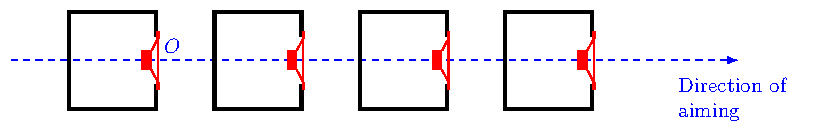
\includegraphics{FIG_1.pdf}
	\caption{\label{fig1}Linear end-fire array with four subwoofers}
\end{figure}

\section{Work to do}
Your work is to design and build a \textbf{scale model} (1 : 10) of a \textbf{directive subwoofer system} for the
concert venue depicted in Fig.~\ref{fig2}. The expected full scale frequency bandwidth is 20 -- 120 Hz yielding a 200 --
1200 Hz bandwidth for the mock-up.

\begin{figure}[!h]
	\centering
	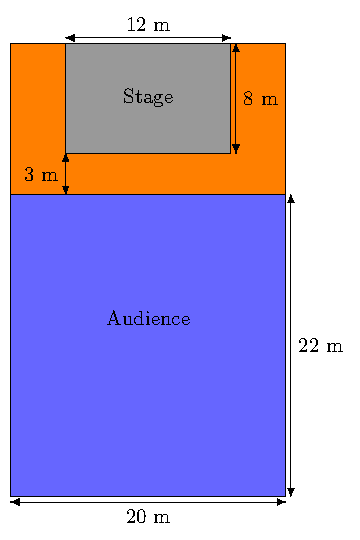
\includegraphics{FIG_2.pdf}
	\caption{\label{fig2}Geometry of the outdoor concert venue (real dimensions)}
\end{figure}

\textbf{Mandatory specifications:}
\begin{itemize}
	\item The system must use 4 identical closed box subwoofers (so 4 small closed box loudspeakers for the mock-up).
	\item The whole system is driven by a mono signal but each single subwoofer can be amplified, filtered or delayed separately.
	\item To save space on the stage, sources must be placed in the orange area of Fig.~\ref{fig2}.
	\item The sources are put on the floor and cannot be hung.
\end{itemize}

\textbf{Free specifications:}
\begin{itemize}
	\item You can use any combination of these 4 subwoofers (loudspeaker spac- ing can be irregular).
\end{itemize}

\textbf{Expected characteristics:} You are asked to design a system that
\begin{itemize}
	\item Has the more constant frequency response in the 200 -- 1200 Hz frequency bandwidth (for the mock-up);
	\item Provides a nearly even coverage of the audience area (low level fluctuations);
	\item That radiates significantly less energy on the stage than on the audience or in the neighborhood.
\end{itemize}

\section{Available equipment}
\begin{itemize}
	\item 4 small closed box systems
	\item A 8 channel USB sound card.
	\item A digital loudspeaker processor (with equalization and delay management)
	\item A 4 channel amplifier
	\item A computer with Matlab and various audio software
	\item Cables
\end{itemize}

\section{Suggested schedule}

In your timetable, you have 12 time slots of 3 hours dedicated to this work
for which you can have access to the project room.Practical work and
measurements must be performed within these slots. If required, you can
also perform simulations or writing work in the free time of your schedule.

\begin{enumerate}
	\item Bibliographic study
	\item Simulation of the chosen geometry with monopoles
	\item Measurement of individual closed box system responses.
	\item Simulation of the system with individual closed box responses.
	\item Building and Measurement of the system in the semi-anechoic room.  (directivity and coverage)
	\item Comparison with theory
	\item Poster design
\end{enumerate}

At the beginning, you can start by simulating the subwoofer behavior by using a monopole formulation:

\begin{equation}
	p = \frac{jk\rho cQ}{4\pi}\frac{-e^{jkR}}{R} \label{eq1}
\end{equation}

In Equation~\ref{eq1}, the time dependence $e^{j\omega t}$ has been omitted. The volume velocity of the source is
denoted $Q$.

\section{Presentation of your work}

You are asked to design a scientific poster design (A0 size). You will be
evaluated both on the poster (scientific work quality, pertinence, conciseness
and clarity of the material printed) and on the oral defense of the material
presented on the poster (15 minutes).

The poster should be printed for the 28\textsuperscript{th} of November. The oral defense is
scheduled on the 1\textsuperscript{st} of December at 2pm.

{\scriptsize
\begin{description}
	\item[Tips for poster design] \url{http://www.cns.cornell.edu/documents/ScientificPosters.pdf}
	\item[Latex templates] \url{http://www.latextemplates.com/cat/conference-posters},
		\url{http://www.brian-amberg.de/uni/poster/},
		\url{http://www-i6.informatik.rwth-aachen.de/~dreuw/latexbeamerposter.php}
	\item[Powerpoint templates]
		\url{http://www.posterpresentations.com/html/free_poster_templates.html},\url{www.wakehealth.edu/Creative/Resources/Tip-Sheets/Creating-Large-Format-Posters-Using-PowerPoint.htm}
\end{description}
}


\section*{References}

\begin{enumerate}
	\item M. Boone, W. Cho \& J. Ih, “Design of a highly directional endf i re loudspeaker array”, J. Audio Eng. Soc., 309-25, 382-92 (2009).
	\item “Forward Steered Arrays in Precision Directivity Speaker Systems”, JBL Technical note vol. 1, Number 28 (2001).
	\item A. Hill, M. Hawkford, A Rosenthal \& G Gand, “Subwoofer positioning, orientation and calibration for large-scale sound reinforcement”, 128th AES convention, London, May 2010.
\end{enumerate}

\end{document}

